\chapter{Predictive Modeling of Adsorption Capacity}
\label{sec:predictive_chapter}

Having established the ability to generate novel polymer structures, this chapter addresses the complementary challenge of predicting their effectiveness. The central predictive task is to estimate the adsorption capacity of a given polymer-molecule pair under specified environmental conditions.

\section{Experimental Setup for the MLP}
\label{sec:mlp_setup}

The Multi-Layer Perceptron employed for capacity prediction is a feedforward neural network with a carefully chosen architecture designed to capture the nonlinear relationships between chemical features and adsorption efficiency. The network consists of an input layer sized to match the dimensionality of the feature vector, multiple hidden layers with progressively decreasing widths (specifically: 16, 8, 4, 4, and 4 neurons in each respective hidden layer), and a single output neuron that produces the predicted capacity value.

The feature vector input to the MLP encompasses all relevant information about the polymer, the target pharmaceutical molecule, and the experimental conditions. This includes the thermodynamic and electronic descriptors extracted as described in Chapter 4: logP and logD values for both polymer and molecule, HOMO-LUMO energies in electron volts, net charges at the relevant pH, and topological descriptors such as TPSA and molecular weight. The Morgan fingerprint representation provides additional structural information, while the initial concentration and water pH encode the experimental context.

Preprocessing of the input features is critical for stable and effective training. The feature vector is scaled using a StandardScaler, which transforms each feature to have zero mean and unit variance. This ensures that features measured in different units (such as energies in eV versus dimensionless logP values) contribute proportionally to the learning process. A separate MinMaxScaler is applied to the target capacity values, mapping them to the range [0, 1] to facilitate gradient-based optimization.

The output activation function requires special consideration. Because adsorption capacity is inherently non-negative, a SoftPlus activation function is applied to the network output. SoftPlus is a smooth, differentiable approximation of the ReLU function, defined as $\text{SoftPlus}(x) = \log(1 + e^x)$. Unlike a linear output, which could theoretically produce negative predictions, SoftPlus guarantees non-negative outputs that are consistent with the physical nature of the target variable.

Training is performed using the Adam optimizer with mean squared error (MSE) as the loss function. The MSE loss is appropriate for regression tasks where larger errors should be penalized proportionally more than smaller errors. The model is trained for a fixed number of epochs with early stopping based on validation loss when a validation set is available.

\section{Addressing the Small Dataset Challenge}
\label{sec:small_dataset}

The limited size of the PDCC dataset presents the most significant challenge for predictive modeling. With only a few hundred experimental observations available, standard machine learning practices that assume abundant data must be adapted. Several strategies were employed to maximize the effective information content of the available data and to obtain reliable performance estimates.

Leave-One-Out Cross-Validation (LOOCV), the extreme case of K-fold cross-validation where the number of folds equals the number of data points, serves as the primary evaluation methodology. Each fold contains a single observation, and the model is trained on all remaining data. While computationally expensive, LOOCV is particularly valuable for small datasets because it maximizes the amount of training data available in each iteration and provides an almost unbiased estimate of generalization error.

In addition to cross-validation, a comprehensive hyperparameter search was conducted to identify the optimal model configuration. The search space included the learning rate, the number of training epochs, the batch size, and the choice of feature subsets. For each configuration, the Q-squared (Q²) statistic was computed from the cross-validation results. The Q² statistic, analogous to the R² coefficient in standard regression, measures the proportion of variance in the target variable that is explained by the model. A Q² value of 1 indicates perfect prediction, while a value of 0 indicates that the model performs no better than predicting the mean of the training data. The Q² statistic is defined as:

\begin{equation}
\text{Q}^2 = 1 - \frac{\sum_{i=1}^{n}(y_i - \hat{y}_i)^2}{\sum_{i=1}^{n}(y_i - \bar{y})^2}
\end{equation}

where $y_i$ is the actual value, $\hat{y}_i$ is the predicted value, $\bar{y}$ is the mean of the observed values, and $n$ is the number of observations.

The dataset augmentation strategies described in Chapter 4 (interpolation and origin point addition) were applied prior to feature extraction. Different augmentation configurations were tested, and the combination that yielded the best cross-validation performance was selected for the final model.

\section{Cross-Validation Results and Performance Metrics}
\label{sec:cv_results}

The hyperparameter optimization process evaluated a wide range of configurations using Leave-One-Out Cross-Validation. The results provide insight into the model's predictive capability under realistic data constraints.

Among the configurations tested, the optimal hyperparameters were identified based on the highest Q² score achieved during cross-validation. The best-performing configuration achieved a Q² score of 0.984 using LOOCV evaluation. This result indicates that the model explains approximately 98.4\% of the variance in the adsorption capacity.

The distribution of Q² scores across different hyperparameter configurations revealed several important findings. Configurations that included the SoftPlus output activation consistently outperformed those using a linear output, confirming the importance of constraining predictions to the physically meaningful non-negative range. The choice of feature subset had a moderate impact on performance, with configurations using the full feature set (including both Polymetrix descriptors and Morgan fingerprints) performing better than those using reduced feature sets.

The interpolation-based data augmentation provided measurable benefits. The configuration using interpolation followed by origin point addition produced the most consistent cross-validation results, suggesting that the augmented data provides a more complete representation of the capacity-concentration relationship near the boundary conditions.

These results were obtained on the augmented dataset; performance on the original, unaugmented data would be expected to be lower.

\begin{table}[htbp]
	\centering
	\caption[LOOCV results across MLP hyperparameter configurations.]{LOOCV results across MLP hyperparameter configurations. Top 10 experiments ranked by Q².\footnote{The complete configuration for each experiment is documented in the corresponding folder under RESULTS/mlp\_experiments/.}}
	\label{tab:q2_leaderboard}
	\begin{tabular}{lccc}
		\toprule
		\textbf{Experiment}                 & \textbf{Q²} & \textbf{MAE} & \textbf{RMSE} \\
		\midrule
		hd\_16\_8\_4\_4\_4                  & 0.984       & 1.499        & 6.485         \\
		hd\_16\_8\_4\_4\_4\_only\_y\_scaler & 0.980       & 1.916        & 7.089         \\
		hd\_16\_8\_4\_4\_4\_mae             & 0.972       & 2.757        & 8.533         \\
		hd\_16\_8\_4\_4\_4\_4\_mae          & 0.918       & 4.558        & 14.518        \\
		hd\_16\_8\_8\_8                     & 0.913       & 2.883        & 14.907        \\
		hd\_16\_8\_4\_4\_4\_4               & 0.904       & 3.555        & 15.655        \\
		hd\_32\_16\_8\_8                    & 0.900       & 3.592        & 15.959        \\
		hd\_8\_8\_8\_8                      & 0.894       & 3.328        & 16.493        \\
		hd\_16\_16\_16                      & 0.888       & 3.387        & 16.926        \\
		hd\_32\_16\_8\_4                    & 0.834       & 4.567        & 20.583        \\
		\bottomrule
	\end{tabular}
\end{table}

\begin{figure}[htbp]
	\centering
	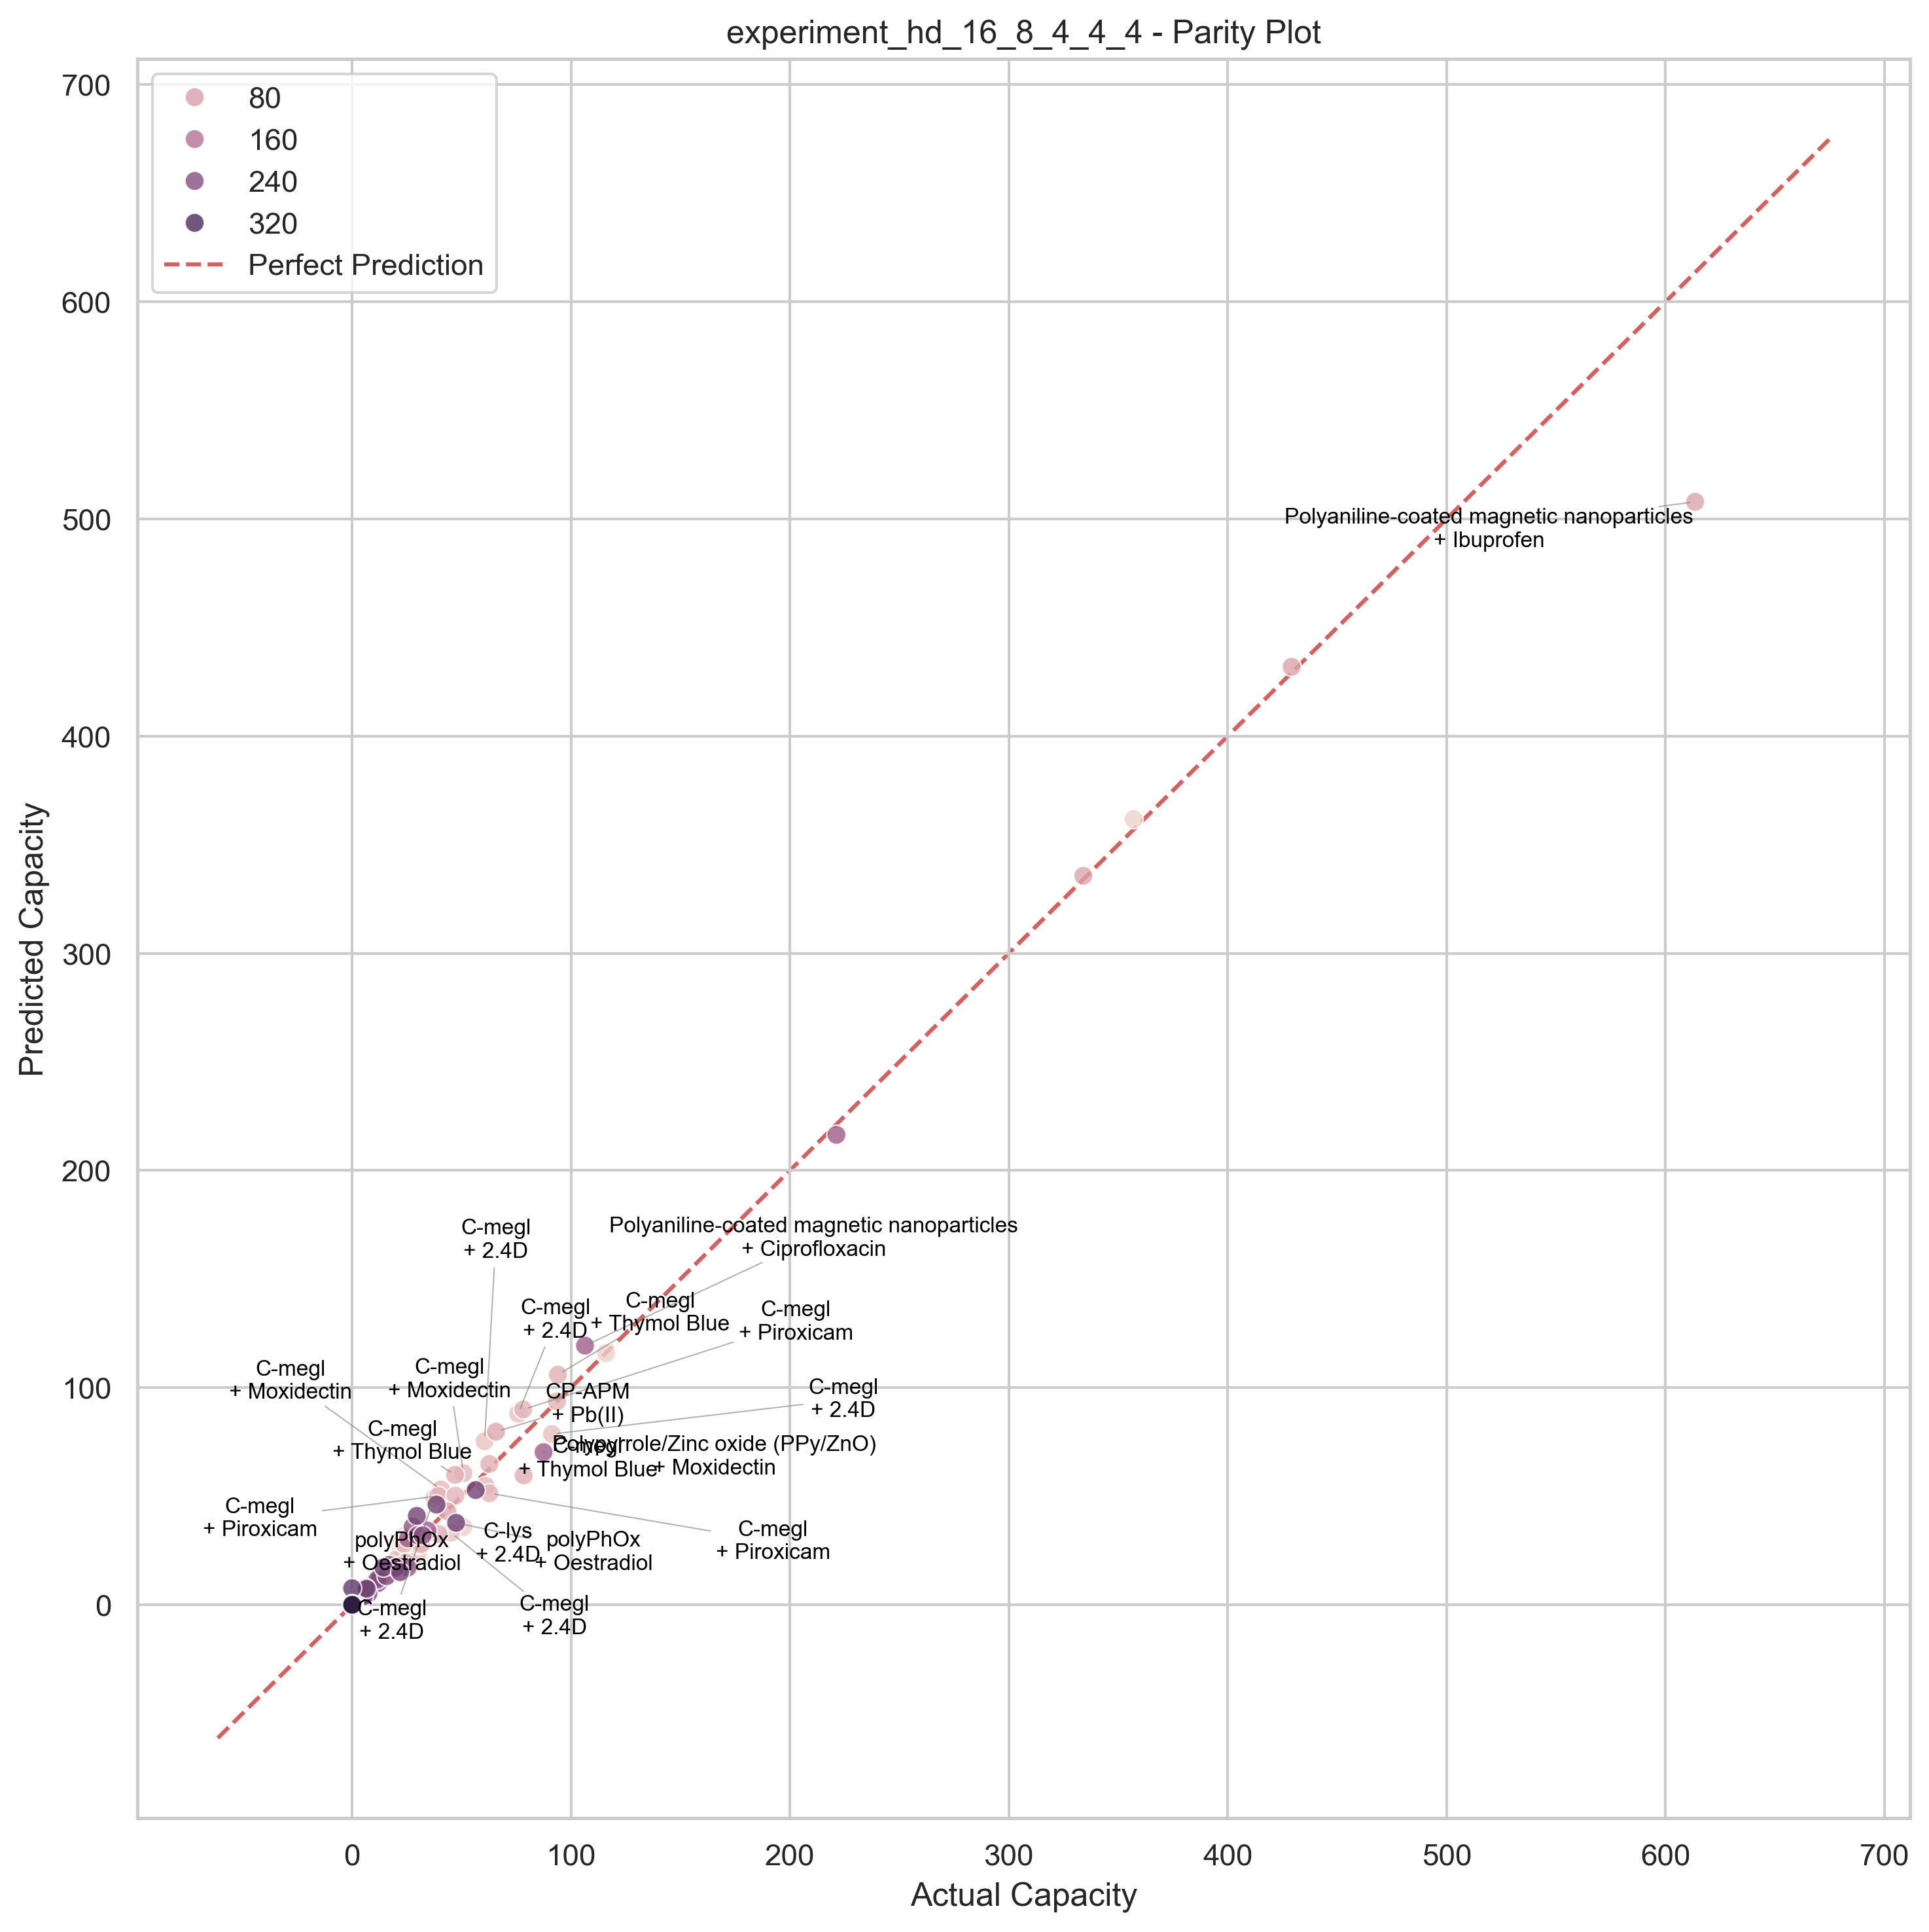
\includegraphics[width=\textwidth]{RESULTS/mlp_experiments/experiment_hd_16_8_4_4_4/parity_plot.png}
	\caption{Parity plot for the optimal MLP configuration (Q² = 0.984). Predicted vs. actual adsorption capacity values.}
	\label{fig:parity_best}
\end{figure}

\begin{figure}[htbp]
	\centering
	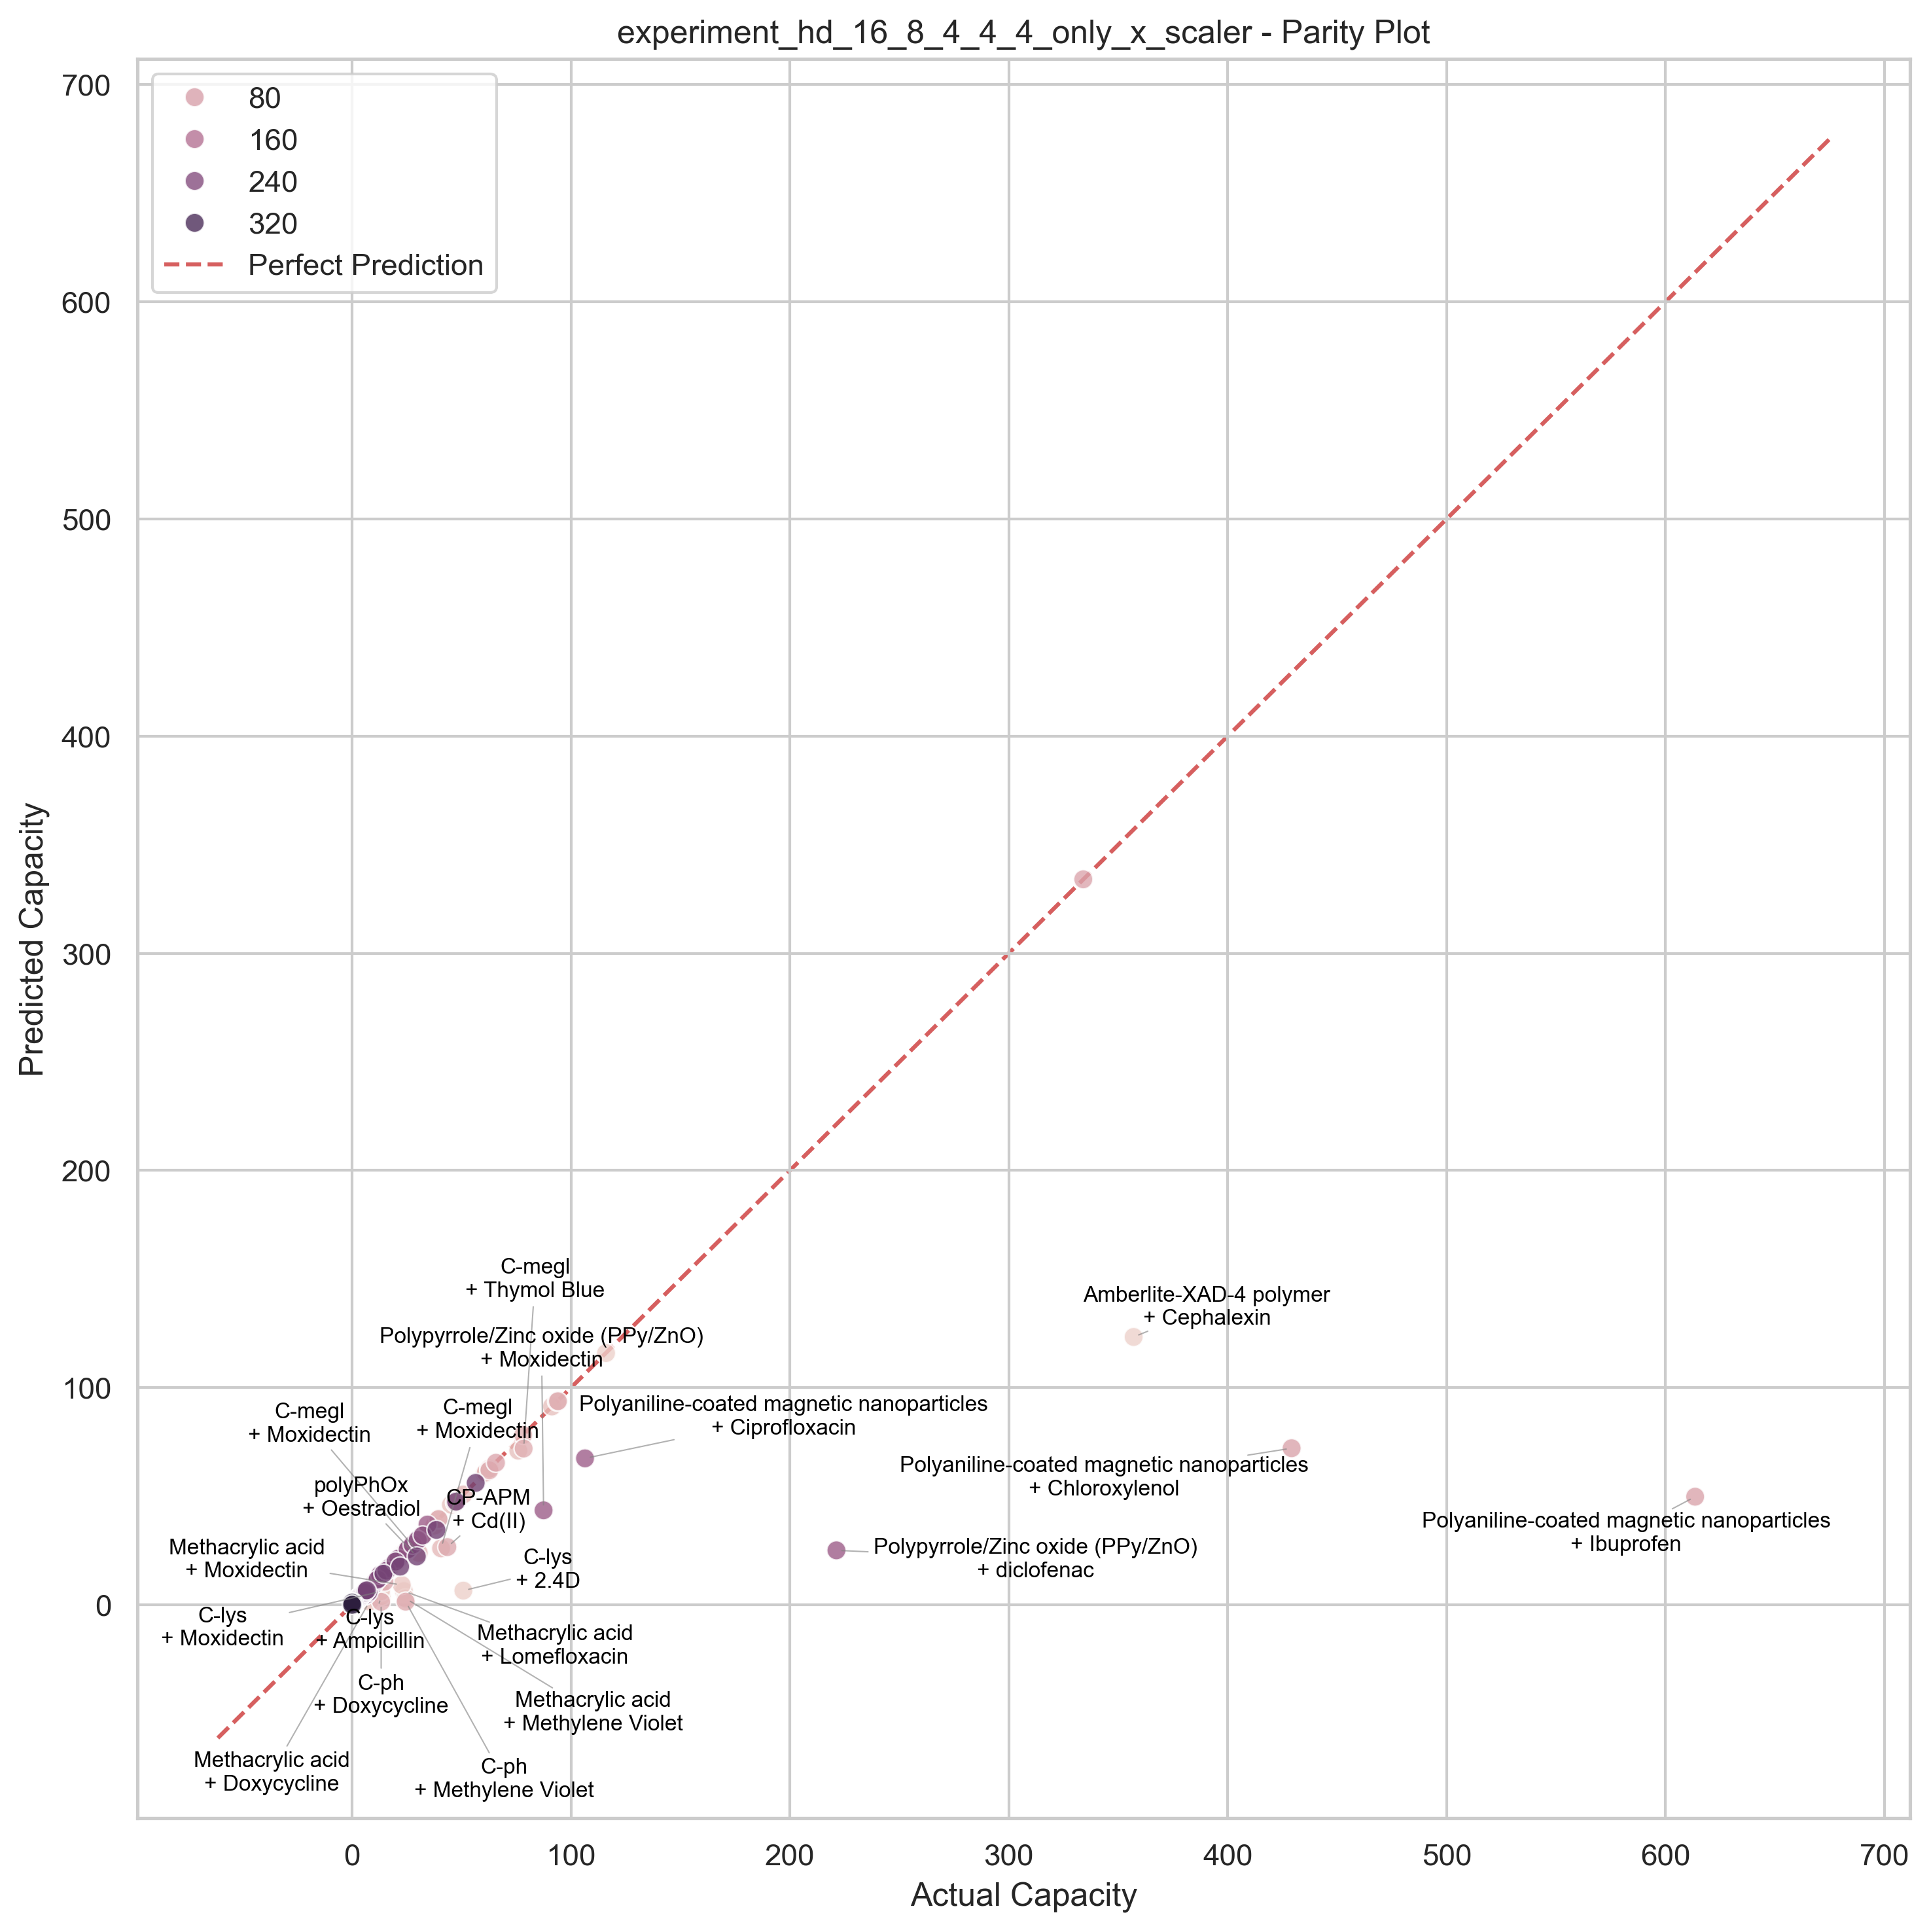
\includegraphics[width=\textwidth]{RESULTS/mlp_experiments/experiment_hd_16_8_4_4_4_only_x_scaler/parity_plot.png}
	\caption{Parity plot for the MLP configuration without Y-scaling (Q² = 0.413). The increased scatter demonstrates the importance of target scaling for prediction quality.}
	\label{fig:parity_no_yscaler}
\end{figure}

\section{Exploratory Clustering Analysis of the PDCC Dataset}
\label{sec:clustering_analysis}

To gain insight into the structure of the PDCC dataset and identify natural groupings among polymer-molecule pairs, an Agglomerative Hierarchical Clustering (AHC) analysis was performed. AHC iteratively merges data points based on their feature similarity, producing a hierarchical structure that can be visualized as a dendrogram. Two complementary visualizations of the clustering results are presented: the dendrogram, which shows the full hierarchical merging process, and a two-dimensional projection via Principal Component Analysis (PCA), which reveals the spatial separation of clusters in reduced dimensionality.

\begin{figure}[htbp]
	\centering
	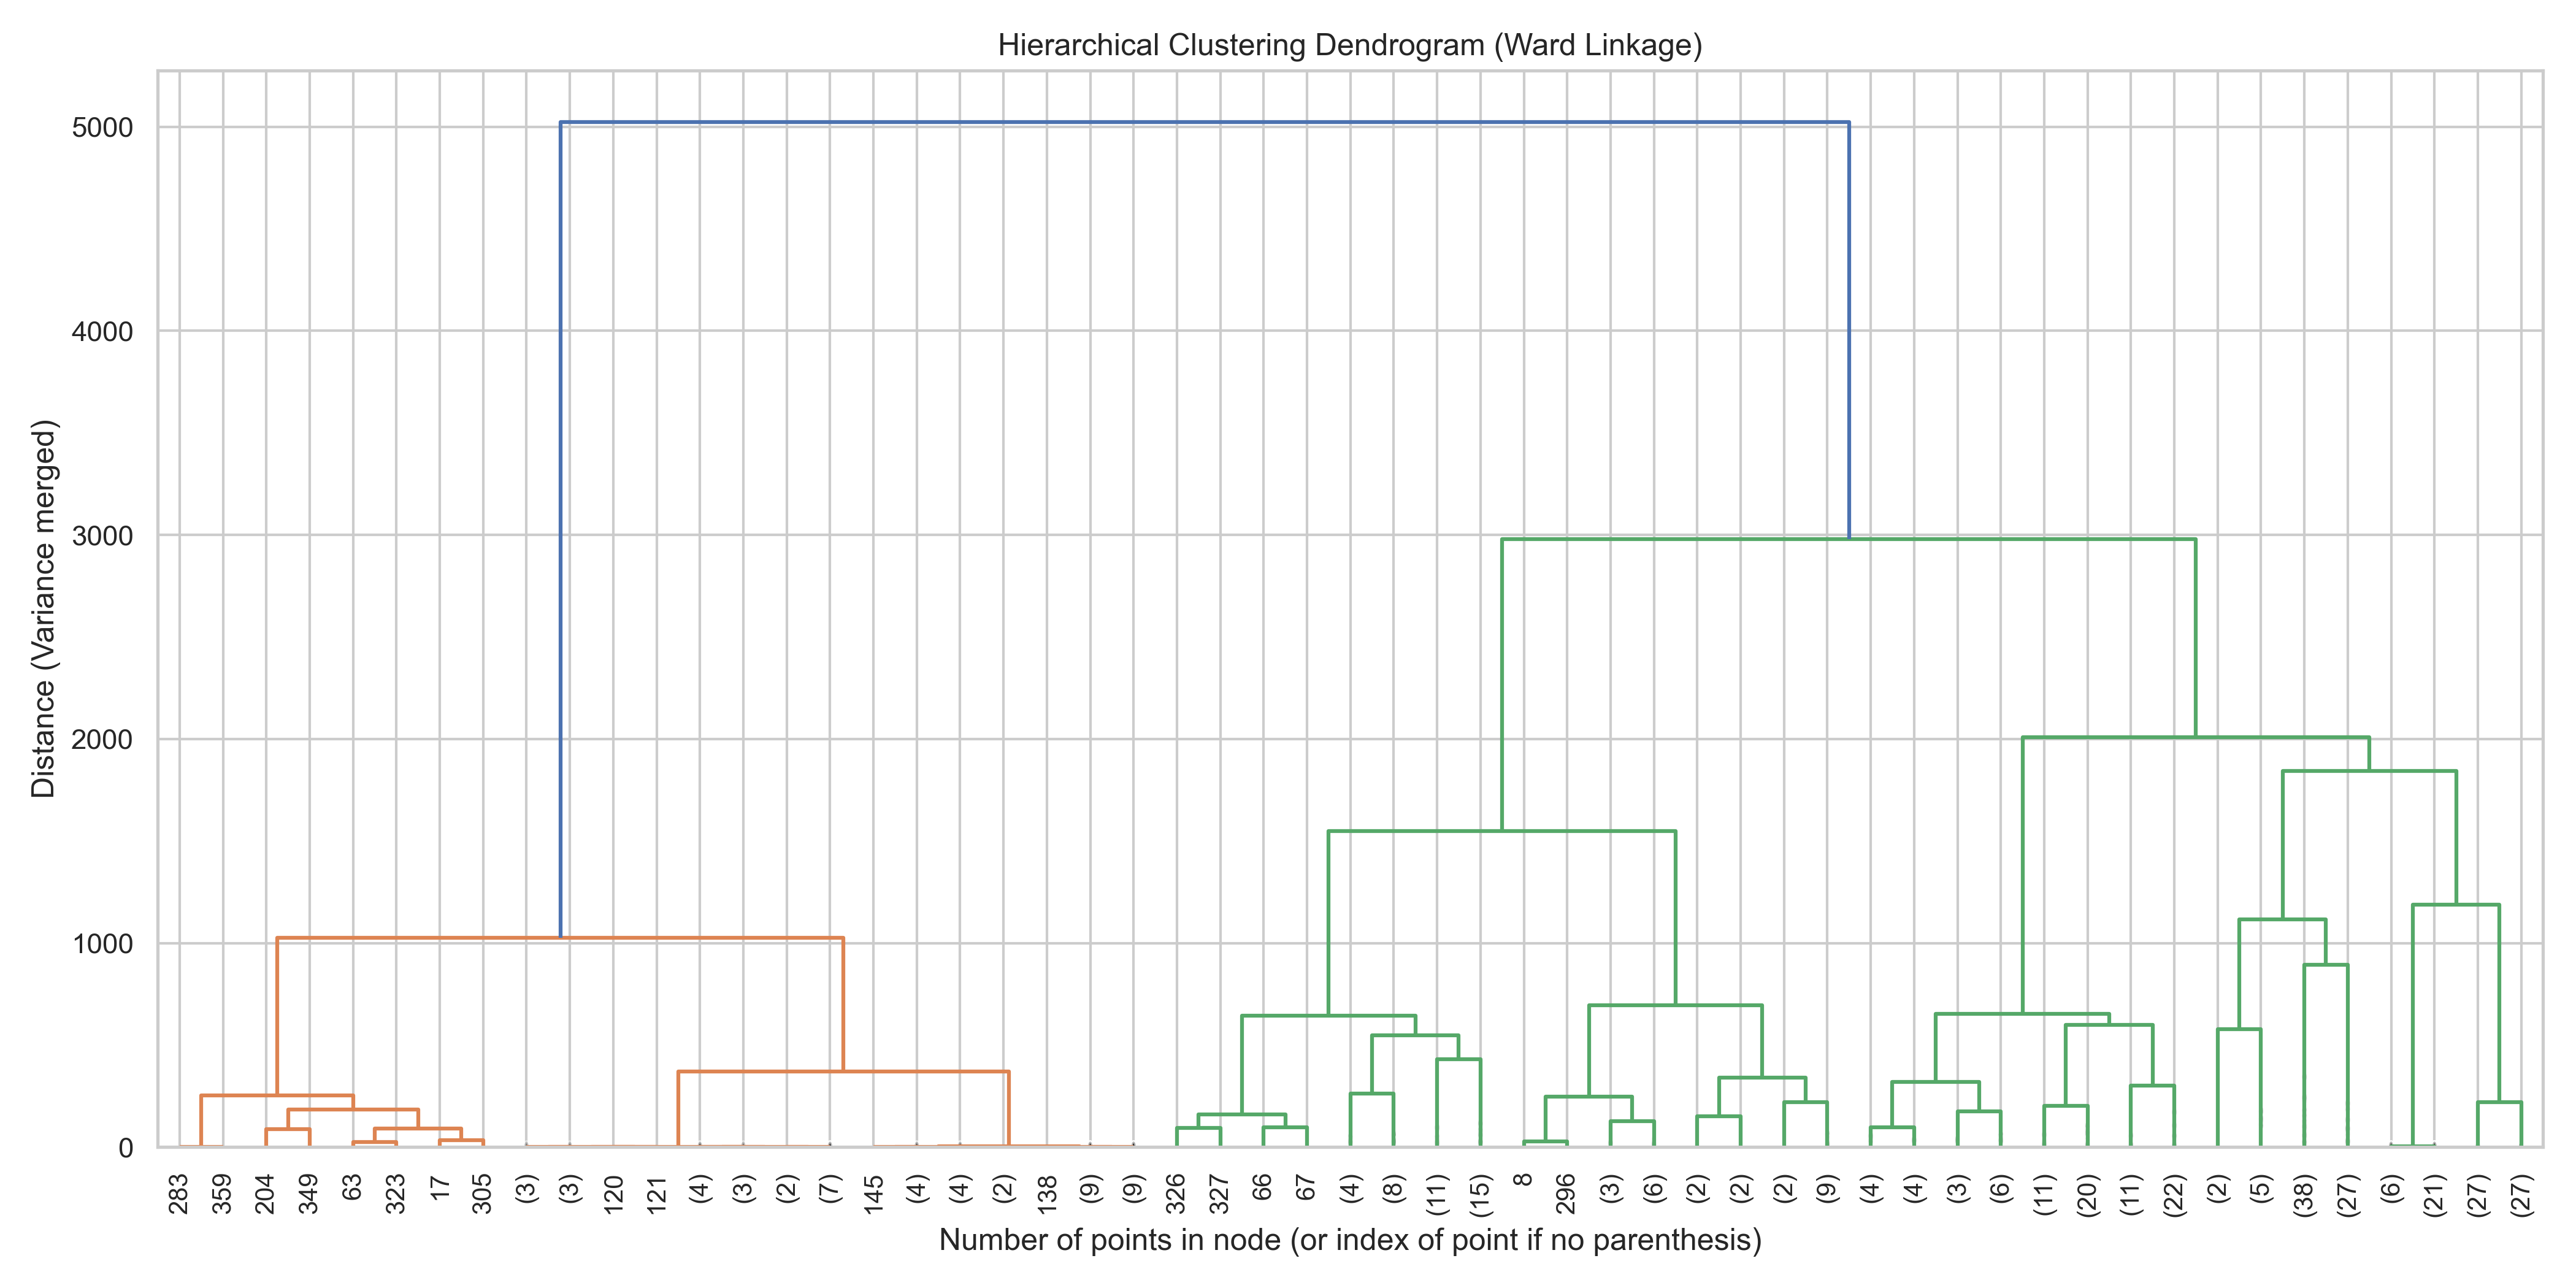
\includegraphics[width=\textwidth]{RESULTS/ahc_clustering/ahc_dendrogram.png}
	\caption{Agglomerative Hierarchical Clustering dendrogram of the PDCC dataset. The y-axis represents the linkage distance; lower merges indicate more similar data points.}
	\label{fig:ahc_dendrogram}
\end{figure}

\begin{figure}[htbp]
	\centering
	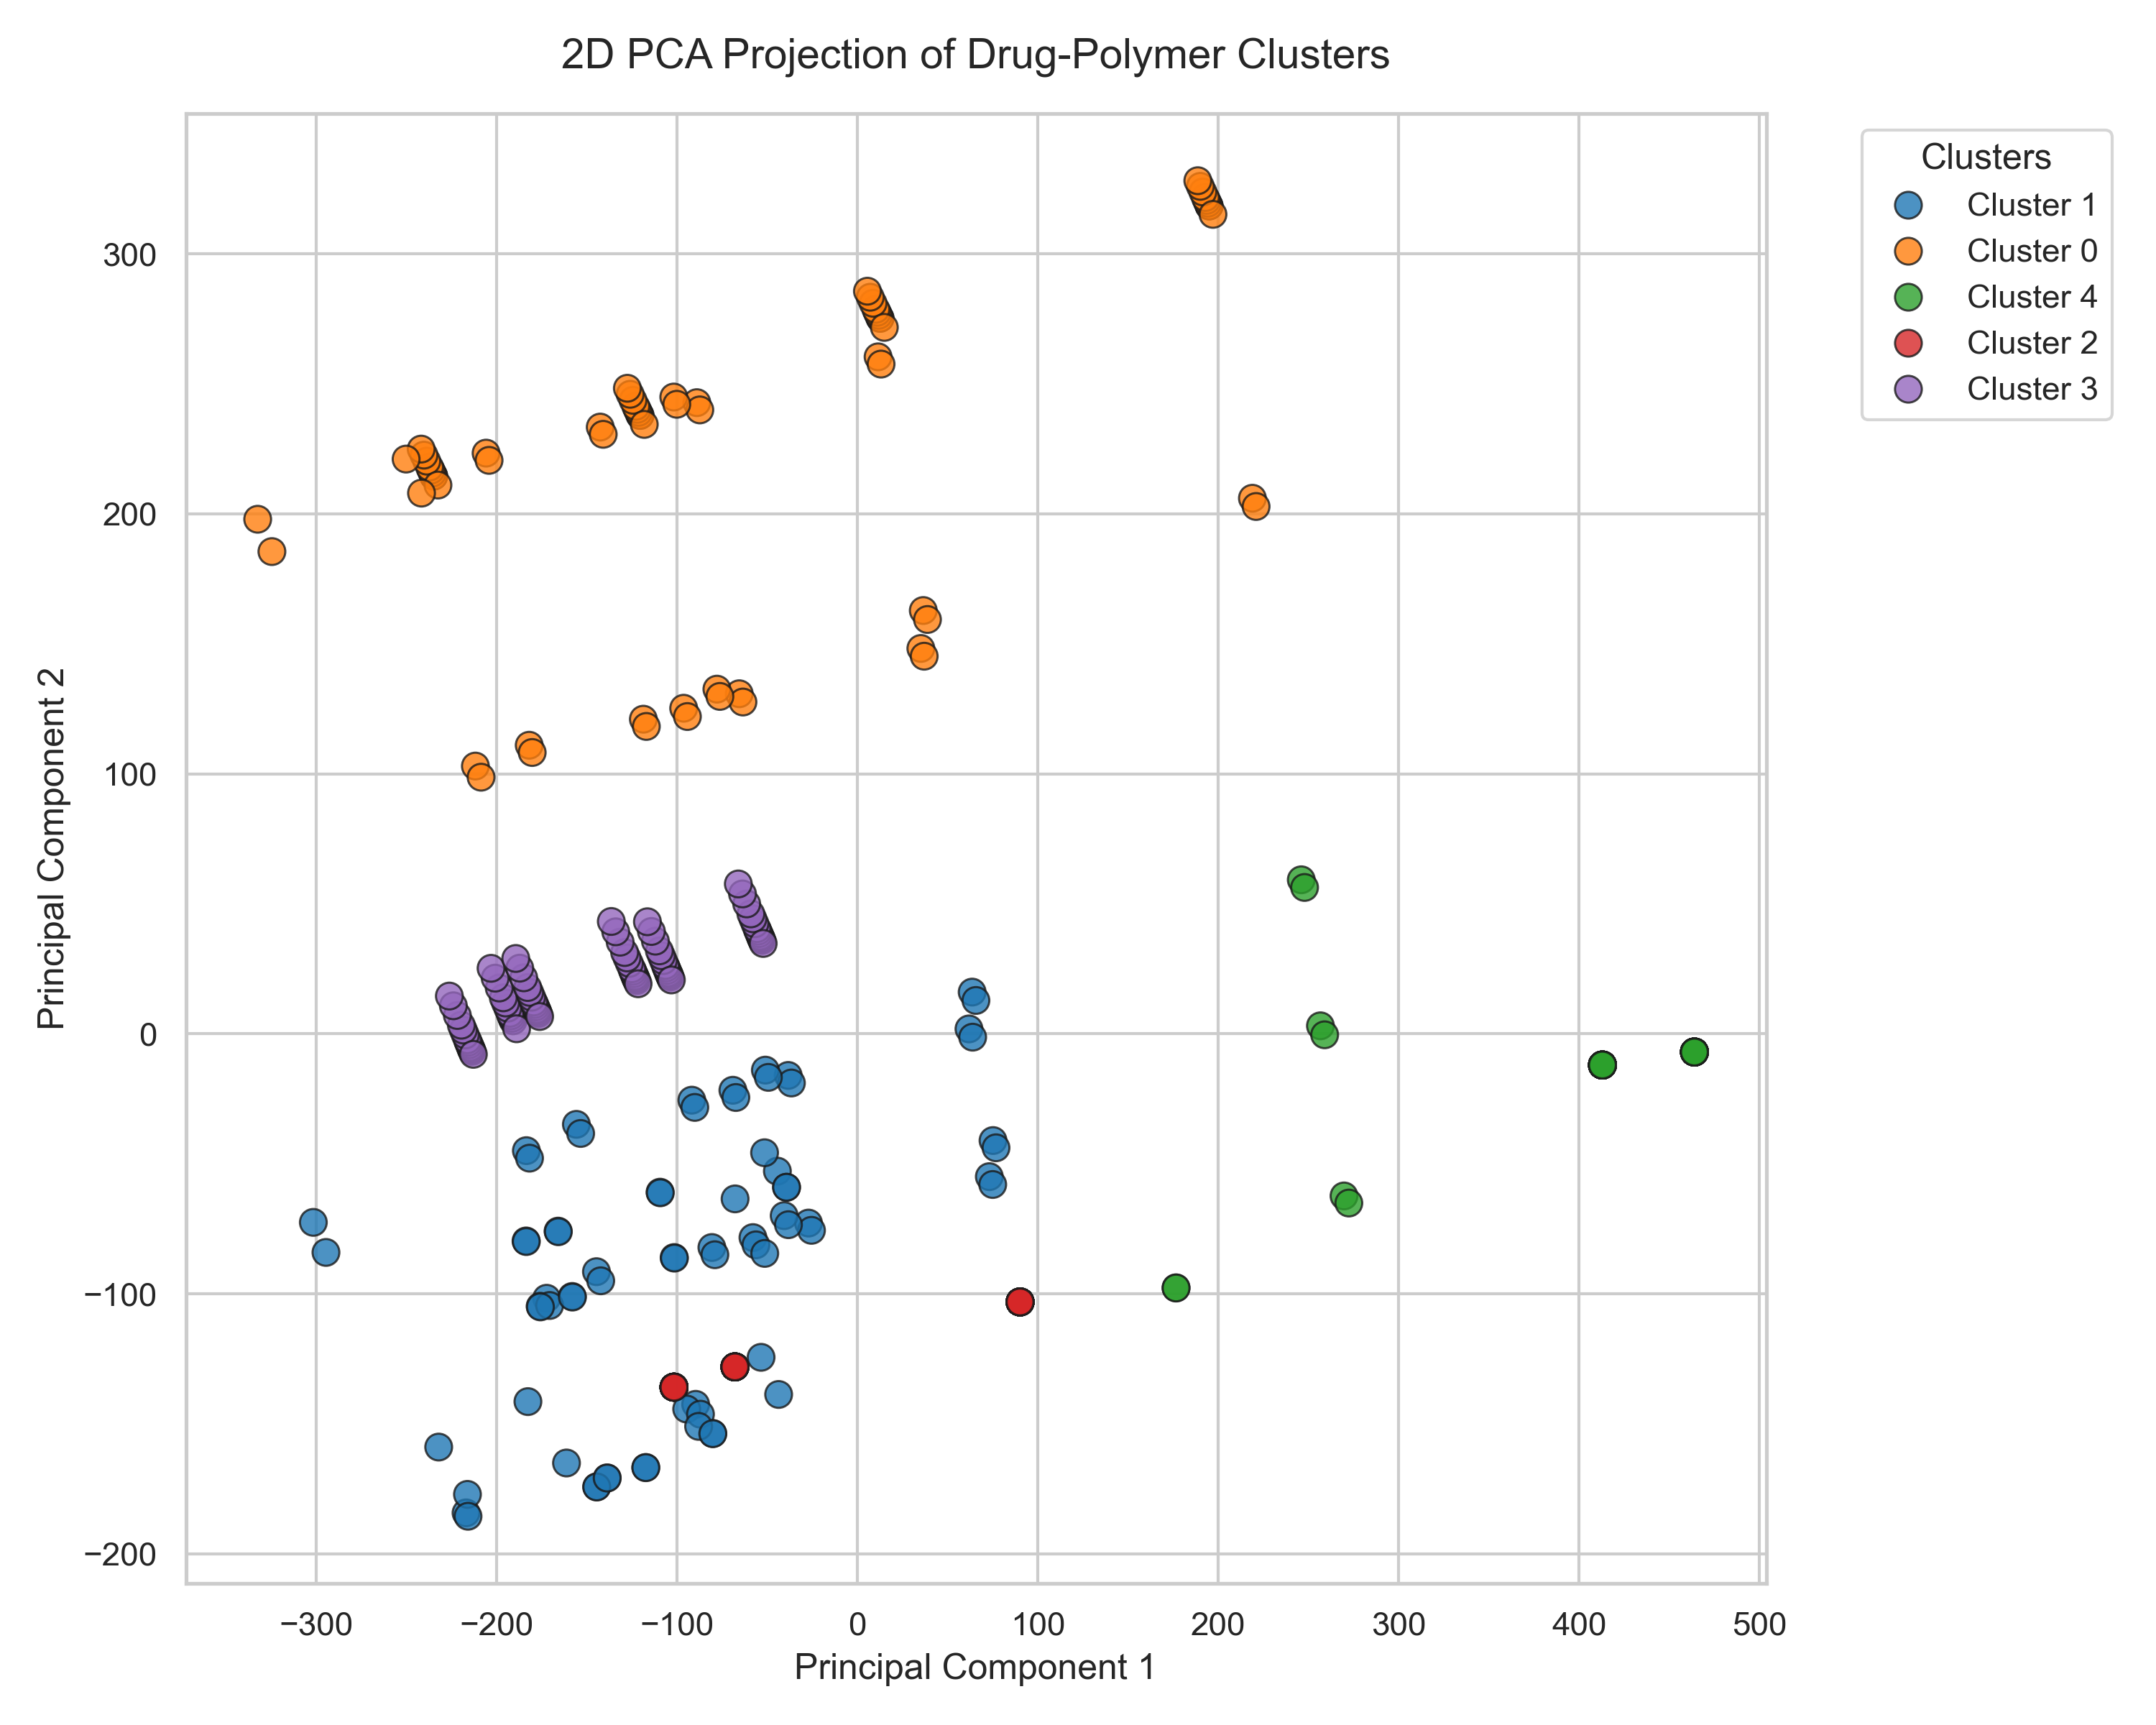
\includegraphics[width=0.75\textwidth]{RESULTS/ahc_clustering/cluster_plot.png}
	\caption{PDCC data projected onto the first two principal components, colored by cluster assignment. Cluster membership reveals groupings driven primarily by polymer molecular weight (PC2) and drug molecular properties (PC1).}
	\label{fig:ahc_cluster_pca}
\end{figure}

\section{Discussion of Model Limitations}
\label{sec:model_limitations}

Despite the encouraging results, several limitations must be acknowledged. The most fundamental limitation is data scarcity. The PDCC dataset contains orders of magnitude fewer observations than typical machine learning benchmarks. Training deep neural networks on such limited data risks overfitting, where the model memorizes specific training examples rather than learning generalizable patterns. While cross-validation provides a measure of generalization performance, the confidence intervals on these estimates are wide due to the small sample size.

The second limitation concerns the representativeness of the training data. The scraped literature reports successful adsorption experiments, potentially introducing publication bias. Polymer-molecule pairs that did not exhibit significant adsorption may be underrepresented or absent from the dataset. A robust predictive model requires data on both successes and failures to learn the boundary between effective and ineffective adsorbents.

The third limitation relates to feature quality. As discussed in Chapter 4, polymer features are computed from capped monomers rather than full polymer chains. This approximation neglects higher-order polymer properties such as chain length distribution, cross-linking density, and three-dimensional conformation, all of which influence adsorption behavior.

\section{Chemical Filtering of Candidate Polymers}
\label{sec:filtering_section}

Complementing the quantitative predictions of the MLP, a set of heuristic filters based on established chemical principles is applied to eliminate polymers that are unlikely to be effective adsorbents. These filters encode domain knowledge about the requirements for successful adsorption in wastewater treatment.

The first filter concerns the partition coefficient (logP) of the polymer. For a polymer to function as an insoluble adsorbent in aqueous solution, it must have a sufficiently high logP value to remain in a solid phase. A minimum logP threshold of 1.5 is applied, ensuring that the polymer remains hydrophobic enough to avoid dissolution while not being so lipophilic that it loses affinity for the aqueous pollutant.

The second filter addresses polar surface area (TPSA). Polymers with higher TPSA values possess more polar functional groups that can engage in hydrogen bonding and electrostatic interactions with pollutant molecules. A minimum TPSA of 60 \r{A}² is required to ensure sufficient polar character for effective binding.

The third and most important filter is based on Frontier Molecular Orbital (FMO) theory. The HOMO and LUMO energies of both the polymer and the target drug determine the nature of their electronic interactions. Two interaction pathways are possible: the polymer acts as an electron donor (using its HOMO) to the drug (acting as an acceptor via its LUMO), or vice versa. The energy gaps for these two pathways are computed as:

\begin{equation}
	\Delta E_1 = |E_{\text{LUMO, drug}} - E_{\text{HOMO, polymer}}|
\end{equation}

\begin{equation}
	\Delta E_2 = |E_{\text{LUMO, polymer}} - E_{\text{HOMO, drug}}|
\end{equation}

The smaller of these two gaps represents the dominant interaction pathway. A smaller intermolecular FMO gap indicates stronger electronic coupling and thus stronger binding. A maximum gap threshold of 4.0 eV is applied, retaining only those polymer-molecule pairs with favorable electronic complementarity.

The fourth filter addresses synthetic accessibility (SA score). A practical wastewater adsorbent must be synthesizable at scale using reasonable chemical methods. The SA score, computed from structural features that affect synthetic difficulty, is constrained to a maximum value of 4.5 on a 1-10 scale.

These filters are applied sequentially after generation and validation, dramatically reducing the number of candidate polymers before they are passed to the predictive model for capacity estimation. The combination of chemical filtering and machine learning prediction provides a balanced approach that leverages both domain knowledge and data-driven pattern recognition.

\section{The Integrated Discovery Pipeline}
\label{sec:discovery_pipeline_section}

The complete computational pipeline integrates generation, validation, filtering, and prediction into an end-to-end workflow for polymer discovery. Given a target pharmaceutical molecule (e.g., aspirin, ibuprofen, or metformin), the pipeline proceeds as follows.

First, the target molecule is converted to SMILES notation using the PubChem database. Second, the generative model produces a batch of candidate polymer P-SMILES strings. Third, invalid and duplicate structures are eliminated through validation. Fourth, the heuristic filters based on logP, TPSA, FMO gaps, and SA score are applied. Fifth, the MLP predicts the adsorption capacity for each surviving candidate. Finally, candidates are ranked by predicted capacity, and those exceeding a specified threshold are returned as promising discoveries.

This pipeline was tested with multiple target molecules, demonstrating its ability to identify candidate polymers with predicted capacities in excess of 1.0 mg/g. Visualization of capacity versus concentration and pH provides additional insight into how the predicted performance varies with experimental conditions, guiding the design of laboratory validation experiments.

\begin{figure}[htbp]
	\centering
	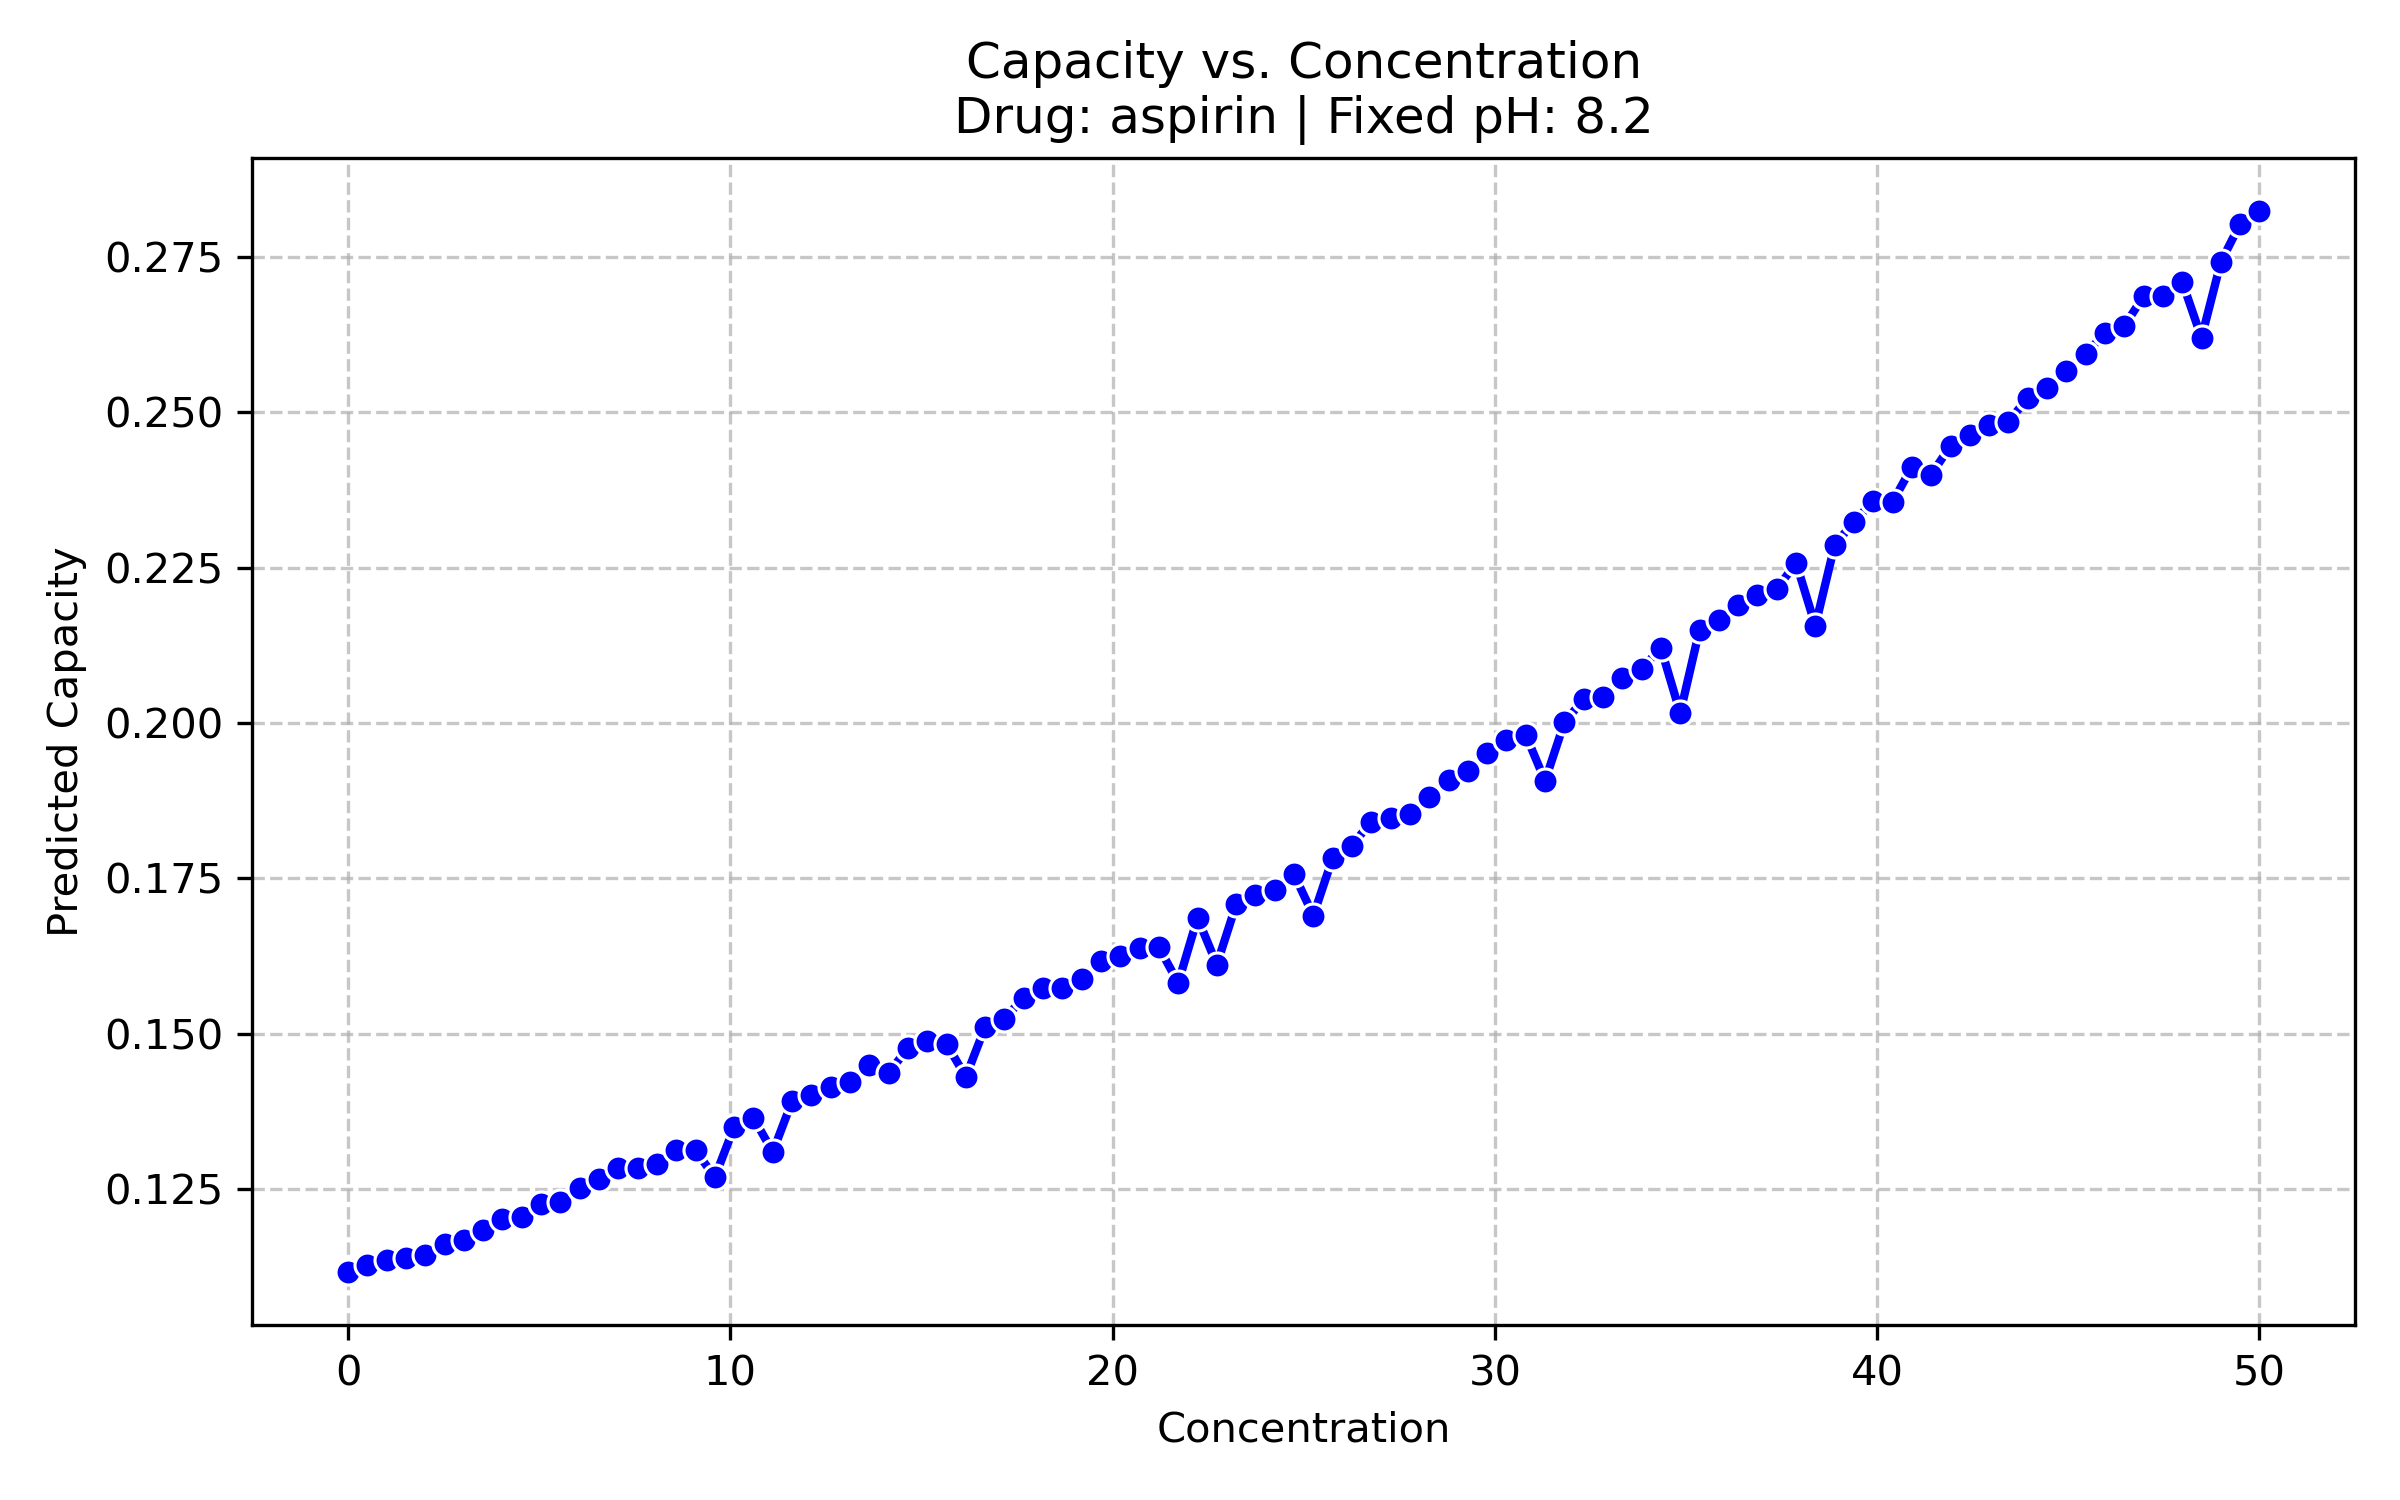
\includegraphics[width=0.75\textwidth]{RESULTS/predicted_capacities/plot_conc_aspirin.png}
	\caption{Predicted adsorption capacity vs. initial concentration for the top-ranked polymer against aspirin.}
	\label{fig:pipeline_conc_aspirin}
\end{figure}

\begin{figure}[htbp]
	\centering
	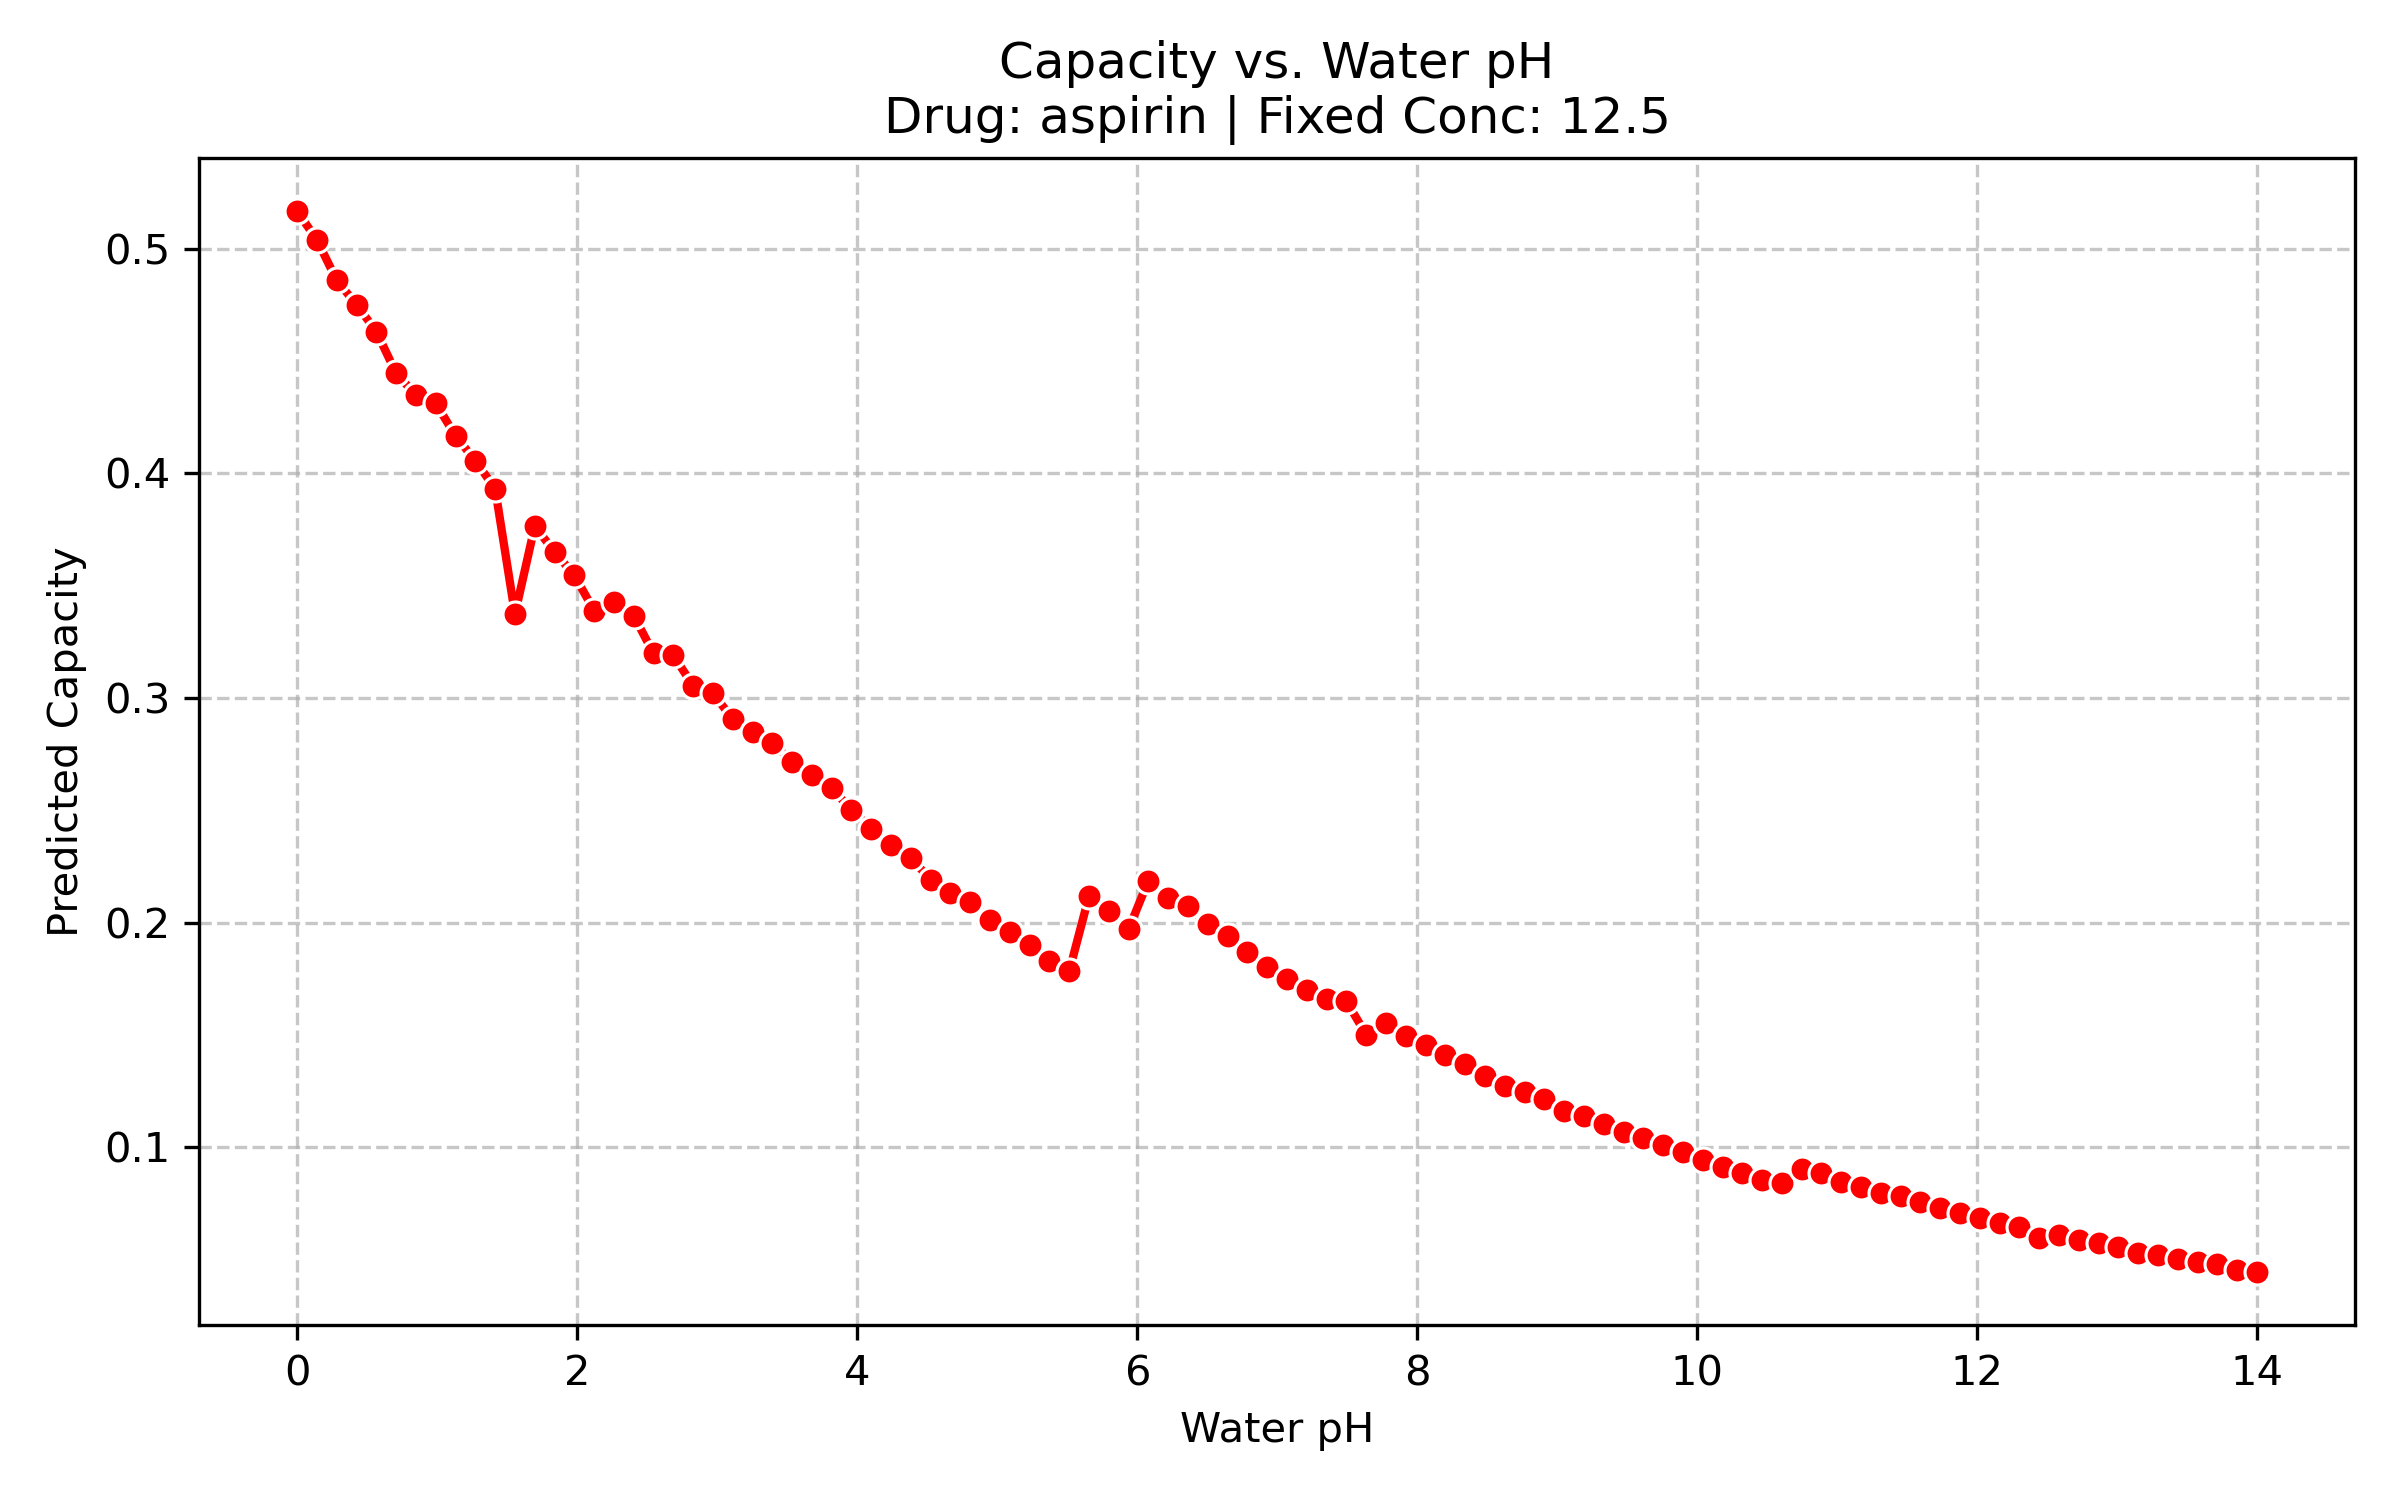
\includegraphics[width=0.75\textwidth]{RESULTS/predicted_capacities/plot_ph_aspirin.png}
	\caption{Predicted adsorption capacity vs. water pH for the top-ranked polymer against aspirin.}
	\label{fig:pipeline_ph_aspirin}
\end{figure}

The pipeline is configurable, allowing adjustment of generation parameters (temperature, batch size), filter thresholds, and the target capacity cutoff. This flexibility enables adaptation to different application contexts, such as targeting different pollutant classes or optimizing for specific environmental conditions.
